% $Header: /cvsroot/latex-beamer/latex-beamer/solutions/conference-talks/conference-ornate-20min.en.tex,v 1.7 2007/01/28 20:48:23 tantau Exp $

\documentclass[10pt]{beamer}



\mode<presentation>
{
  \usetheme{Berkeley}
  % or ...

  \setbeamercovered{transparent}
  % or whatever (possibly just delete it)
}


\usepackage[english]{babel}
% or whatever

\usepackage[latin1]{inputenc}
% or whatever

\usepackage{times}
\usepackage{graphicx}

\usepackage{tikz}
\usepackage{lineno}
\usepackage[english]{babel}
\usepackage{seqsplit}
\usepackage[nottoc]{tocbibind} 
\usepackage[utf8]{inputenc}
\usepackage{amsmath}
\usepackage{amssymb}
\usepackage{amsthm}
% \newtheorem{theorem}{Theorem}
% \newtheorem{lemma}[theorem]{Lemma}
% \newtheorem{corollary}{Corollary}[theorem]
% \newtheorem{definition}{Definition}
% \newtheorem{proposition}{Proposition}
% \newtheorem{example}{Example}

\title[Part C Dissertation] % (optional, use only with long paper titles)
{Extensions of number fields with small ramification}

\subtitle
{}

\author % (optional, use only with lots of authors)
{Samuel Bodansky}


\institute % (optional, but mostly needed)
{
  University of Oxford
  }
.

\date % (optional, should be abbreviation of conference name)
{February 2019}
\setbeamertemplate{sidebar right}{}
\setbeamertemplate{footline}{%
\hfill\usebeamertemplate***{navigation symbols}
\hspace{1cm}\insertframenumber{}/\inserttotalframenumber}

\begin{document}

\begin{frame}
  \titlepage
\end{frame}
\begin{frame}{Contents}
\tableofcontents
\end{frame}

\section{Goal}
\begin{frame}{Aim of Project}
Goal: For a given number field K, what is the maximal unramified extension $K^{ur}$ of K is and also what is the structure of $G_K^{ur}$ is.

\end{frame}

\begin{frame}{Notation}
Here is a summary of relevant notation for this talk. 
\end{frame}
\section{Class Field Theory}
\begin{frame}{CFT Definitions}
    \begin{definition}
    A prime ideal $\mathfrak{p}$ in $\mathcal{O}_K$ factors in an extension L of K as
\par
$\mathfrak{p}\mathcal{O}_L=\mathfrak{B}_1^{e_1}...\mathfrak{B}_m^{e_m}$, where $\mathfrak{B}_i$ are ideals in $\mathcal{O}_L$ intersecting $\mathcal{O}_K$ at $\mathfrak{p}$. Each $e_i\geq1$ and if $e_i>1$ for some i then we say that $\mathfrak{p}$ ramifies in L. If $e_i=1$ for all i then we say $\mathfrak{p}$ splits in L.
    \end{definition}
    \begin{definition}
    Let H be a subgroup of the class group C of K. A finite unramified abelian extension L of K is said to be a $\textit{class field}$ for H if the prime ideals of K splitting in L are exactly those in $\tilde{H}$.
    \end{definition}
    
\end{frame}
\begin{frame}{Key Result about Unramified Extensions}
The following theorem will allow us to define $K^{ur}$:
    \begin{theorem}
The compositum of two finite unramified extensions of K is also unramified, and so the union $K^{ur}$ of all unramified extensions is also an unramified extension of K. The residue field $\tilde{k}$ of $K^{ur}$ is an algebraic closure of the residue field k of K.
\end{theorem}

\end{frame}
\begin{frame}{Proof of Theorem}
    \begin{proof}
    Suppose K is a number field and $L,\tilde{L}$ are extensions of K. Let $\mathfrak{p}$ be an ideal unramified in $L$ and $\tilde{L}$. Let $P$ be a prime lying over $\mathfrak{p}$ in $L\tilde{L}$. Let $M$ be the minimal normal extension of $L\tilde{L}$, i.e. the normal closure. Suppose $Q$ is a prime in $M$ lying over $P$, then we have 
    \begin{equation}
        \mathfrak{p}\subseteq P \subseteq Q
    \end{equation}
    Let $E=E(Q|\mathfrak{p})$ denote the inertia group of $Q$ at $\mathfrak{p}$. Since $\mathfrak{p}$ is unramified in $L$ and $\tilde{L}$, it follows that $Q \cap \mathcal{O}_L$ and $Q \cap \mathcal{O}_\tilde{L}$ are unramified in $L$ and $\tilde{L}$ respectively. But the inertia field $M^E$ is the largest field in which $\mathfrak{p}$ is unramified, so it follows that $L\subseteq M^E$ and $\tilde{L} \subseteq M^E $, whence $L\tilde{L}\subseteq M^E$ and $\mathfrak{p}$ is unramified in $L\tilde{L}$.
\end{proof}

\end{frame}
\section{$\mathbb{Q}$,P-adics and Cyclotomics}
\subsection{Examples in $\mathbb{Q}$}
\begin{frame}{Extensions of $\mathbb{Q}$}
    \begin{theorem}
     Suppose that K be a field extension of $\mathbb{Q}$ with discriminant D. Then a prime p
ramifies in K if and only if $p|D$.   
    \end{theorem}
    \begin{corollary}
A field extension K of $\mathbb{Q}$ ramifies at precisely one prime iff the absolute value of disc(K) is a prime power.
\end{corollary}
\begin{example}
    Suppose $f(x)=x^5-5x^4-2x^3+x^2-3x+1$, and K is the splitting field of f over $\mathbb{Q}$. Then $disc(K)=-3442951=151^3$ and so 151 is the only prime which ramifies in K over $\mathbb{Q}$. Note that f(x) is an irreducible quintic with precisely three real roots, meaning that $\Gamma(K/\mathbb{Q})\cong\ S_5$ and K is an unsolvable extension of $\mathbb{Q}$.
\end{example}
\end{frame}
\subsection{P-adics and Cyclotomics}
\begin{frame}{P-adics results}
\begin{block}{P-adics}
Suppose $\zeta$ is an $n_{th}$ root of unity. Let K be a number field, $L=K(\zeta)$. Let $\mathcal{O}_L,\mathcal{O}_K$ be their respective valuation rings and $\lambda,\kappa$ be their respective residue class fields. \begin{proposition}
L is a degree n unramified extension of K.
\end{proposition}

Suppose now that $\zeta$ is a primitive n-th root of unity, with $n=kp^{m}$ where k is prime to p. We have the following inclusions:
\end{block}
\begin{example}[Field Inclusions]
      $\mathbb{Q}_{p}=K\subseteq K^{tur}=K(\zeta_k)\subseteq K^{ur} = K^{tur}(\zeta_{p})\subseteq K(\zeta_n)$
\end{example}
\end{frame}
\begin{frame}{Maximal Unramified Extension of P-adic}
    We first use the following lemma 
    \begin{lemma}
Suppose p is a prime and gcd(n,p)=1. Then there exists $m\in\mathbb{N}$ such that $n|p^m-1$.
\end{lemma}
We then have the following:  \begin{theorem}
    Let $K=\mathbb{Q}_p$. Then $K^{ur}$ is K adjoined with all roots of unity with order prime to p. 
\end{theorem}

\end{frame}
\begin{frame}{Cyclotomics Results}
    \begin{theorem}
    Let $\zeta$ denote the $p^m-th$ root of unity, 
    Then we have the following results:
    \begin{enumerate}
        \item $[\mathbb{Q}_{p}(\zeta):\mathbb{Q}_p]$ is totally ramified with degree $(p-1)p^{m-1}$
        \item $\Gamma(\mathbb{Q}_{p}(\zeta):\mathbb{Q}_p)\cong (\mathbb{Z}/p^{m}\mathbb{Z})^{*}$
        \item $\mathbb{Z}_{p}(\zeta)$ is the valuation ring of $\mathbb{Q}_{p}(\zeta)$
        \item $1-\zeta$ is a prime element of $\mathbb{Z}_{p}(\zeta)$ with $N(1-\zeta)=p$
    \end{enumerate}
\end{theorem}
\end{frame}
\section{Hilbert Class Field}
\begin{frame}{Definition of Hilbert Class Field}
    \begin{definition}
The \textbf{class field} of the trivial subgroup of C(K) is called the Hilbert class field of K. 
\end{definition}
\begin{enumerate}
    \item It is maximal abelian extension, L of K unramified at all primes of K. 
    \item  The degree of its extension over K is equal to the class number of K, 
    \item Its Galois group is isomorphic to the ideal class group of K, taking Frobenius elements as prime ideals of K.
    \item If K is a unique factorisation domain then K is equal to its own Hilbert class field. 
\end{enumerate}
\end{frame}
\begin{frame}{Examples of Hilbert Class Fields}
    \begin{example}
    Suppose K=$\mathbb{Q}$. Then K is its own Hilbert class field. 
\end{example}
\begin{example}
    Suppose $K=\mathbb{Q}[\sqrt{-5}]$, and take $L=\mathbb{Q}[\sqrt{-1},\sqrt{-5}]$. L is an unramified degree 2 extension of K and so the Hilbert class field of K is $K[\sqrt{-1}]$.
\end{example}
\begin{example}[Hasse]
    Suppose $K=\mathbb{Q}[\sqrt{-31}]$ with class number 3. Let L be its Hilbert class field. Then L is defined by a root of the polynomial \begin{equation}
        x^3+\frac{3+\sqrt{-31}}{2}x^2+\frac{-3+\sqrt{-31}}{2}x -1 =0.
    \end{equation}
\end{example}
\end{frame}
\begin{frame}{Hilbert Class Field Applications Theorem}
    \begin{theorem}
Theorem: Let L be the Hilbert class field of $K=\mathbb{Q}(\sqrt{-n})$, where n is squarefree, $n\not\equiv 3(4)$, so that
\begin{equation}
    \mathcal{O}_K=\mathbb{Z}(\sqrt{-n})
\end{equation}
Assume that p is an odd prime not dividing n, and that x,y are integers. Then
$p=x^2+ny^2 \Longleftrightarrow$ p splits completely in L.
\end{theorem}
\end{frame}
\begin{frame}{Primes of the form $x^2+ny^2$}
    \begin{corollary}
Suppose $K=\mathbb{Q}{\sqrt{-n}}$ n is positive,squarefree, $n\not\equiv 3(4)$, so that $d_K=-4n$. If p is an odd prime not dividing n, then
\begin{equation} p=x^2+ny^2 \Longleftrightarrow p\:splits\:completely\:in\:the\:Hilbert\:class\:field\:of\:K.
\end{equation}
Hence the primes of the form $x^2+ny^2$ characterise the Hilbert Class field of $\mathbb{Q}(\sqrt{-n})$.
\end{corollary}
\end{frame}
\section{Bounds on Discriminants}
\begin{frame}{Minkowski Bounds}
Minkowski's theorem bound shows that if K is a number field with $r_1$ real and $2r_2$ complex conjugate fields, and $n=r_1+2r_2$ is the degree of the field, then 
\begin{equation}
rd_K\geqslant (\frac{\pi}{4})^{\frac{2r_1}{n}}\frac{n^2}{n!^{\frac{2}{n}}}
\end{equation} 
As $n\rightarrow \infty$, Stirling's formula can give a bound that
\begin{equation}
    rd_K\geqslant e^2 = 7.39
\end{equation}
\end{frame}
\begin{frame}{Odlyzko's Bounds}
    Odlyzko's Bound improved on the bounds for Minkowski for the discriminant of a number field. It can be stated as  
\begin{equation}
rd_K\geqslant 60^{\frac{r_1}{n}}22^{\frac{r_2}{n}}+o(1)\:as\:n\rightarrow \infty   
\end{equation}
Furthermore, under the assumption of the Generalised Riemann Hypothesis, 
this bound can be improved by replacing the numbers 60 and 22 by 188 and 41 respectively. 
\end{frame}
\begin{frame}{Using these Bounds}
Following Yamamura write this bound function as $B(n,r_1,r_2)$.
\begin{theorem}
Suppose that H is a positive integer, and L is an unramified normal extension of K of degree M. Here are two possible cases that can occur:
\begin{enumerate}
    \item If \begin{equation}
        rd_K<B(H.m.n,H.m.r_1,H.m.r_2)
    \end{equation}
    then $[K^{ur}:L]<H$ and $h(L)<H$. Indeed if H=2 then $K^{ur}=L$.

    \item If
        $h(L)=1$ and H=60 then again $K^{ur}=L$.
\end{enumerate}
\end{theorem}
\end{frame}
\section{Infinite Unramified Extensions}
\begin{frame}{The Hilbert p-class Field: Definitions}
    \begin{definition}
A \textbf{p-group} is a group in which every element has order equal to a power of p.
\end{definition}
\begin{definition}
A \textbf{Hilbert p-class field} $H_K^{p}$ of a number field $K$ is the maximal unramified abelian p-extension of K.
\end{definition}
\begin{definition}
A \textbf{Hilbert p-class field} $H_K^{p}$ of a number field $K$ is the maximal unramified abelian p-extension of K, with the \textbf{p-class field tower} defined in a similar way to the definition of the Hilbert tower. 
\end{definition}
\end{frame}
\begin{frame}{The Hilbert p-class Field and Finite Extensions}
    \begin{Theorem}
If any p-class field tower over K is infinite, then the class field tower is also infinite. If the p-class tower terminates, then $H_{K_\infty}^{p}$ is a finite field extension of K and $\Gamma(H_{K_\infty}^{p}/K)$ is a p-group.
\end{Theorem}
Note that the converse to the first part of the above needn't hold; take $\mathbb{Q}(\sqrt{-239},\sqrt{4049})$. Then this biquadratic field extension of $\mathbb{Q}$ has an infinite class field tower, but all p-class field towers are finite. 
\end{frame}
\begin{frame}{Golod and Shafaverich}
    \begin{theorem}
    Let G be a finite p-group, and define $d=dim_{\mathbb{F}_{p}}H^1(G,\mathbb{F}_p)$, $r=dim_{\mathbb{F}_{p}}H^2(G,\mathbb{F}_p)$. 
    Then $r>d^2/4$.
\end{theorem}
\begin{theorem}
    Let $G = \Gamma(H_{K_{\infty}}^{p}/K)$ where K is an imaginary quadratic number field. If G is finitely generated as a pro-p group, then
$r-d\leq 1 $. If p is an odd prime, r=d.
\end{theorem}
The above inequalities give a contradiction for $d \geq 5$ if all such G are assumed to be finite p-groups.
\end{frame}
\begin{frame}{Infinite p-class Tower Examples}
\begin{example}
    Define $K=\mathbb{Q}(\sqrt{-3.5.7.11.19.23})$. Then 6 odd primes ramify in K over $\mathbb{Q}$, and so K has an infinite 2-class field tower. 
\end{example}
\begin{example}[Schoof]
$\mathbb{Q}(\sqrt{-191.773})$ has an infinite 2-class field tower. There are infinitely many real quadratic number fields of the form $\mathbb{Q}(\sqrt{p_1.p_2})$ with $p_1$ and $p_2$ prime, possessing infinite class field towers. 
\end{example}
\end{frame}
\section{Infinite unramified extensions}
\begin{frame}{Example of Unsolvable Unramified Extension}
Let K be a class field with trivial class group, i.e. h(K)=1. Then K has no abelian (and hence no
solvable) non-trivial unramified Galois extension. Despite this, K may have a non-solvable unramified extension. Brink gives 
\begin{equation}
   K=\mathbb{Q}(\sqrt{29},\sqrt{4967}) 
\end{equation}
\begin{equation}
   L=split(x^7 - 11x^5 + 17x^3 - 5x + 1,\mathbb{Q}[x])
\end{equation}
Then K has class number 1 and L is a PSL(2, 7)-extension of K.
Maire showed that there exist biquadratic number fields with class number one with an infinite unramified extension.
\end{frame}
\begin{frame}{Finding a Field with Class Number 1 and Infinite Unramified Extension}
    \begin{theorem}[Brink]
Suppose that \begin{enumerate}
    \item $f\in \mathbb{Z}[x]$ is an irreducible quintic with five real roots
    \item $D=\Delta(f)$ is prime and $\mathbb{Q}(\sqrt{L})$ has class number 1
    \item p and q are two primes such that $\mathbb{Q}(\sqrt{p.q})$ has class number 1 and $\mathbb{Q}(\sqrt{(D.p.q})$ has class number 2.
    \item f has five simple roots modulo p and f factors modulo q into polynomials of degrees, as a tuple $\mu$ of the form (1,1,1,1,1),(1,1,1,3),(1,2,2) or (1,1,3).
\end{enumerate}
Then the field $L=\mathbb{Q}(\sqrt{D},\sqrt{p.q})$ has class number 1 and infinite unramified extension.
\end{theorem}
\end{frame}
\begin{frame}{Field Extension Diagram}
  \begin{center}
    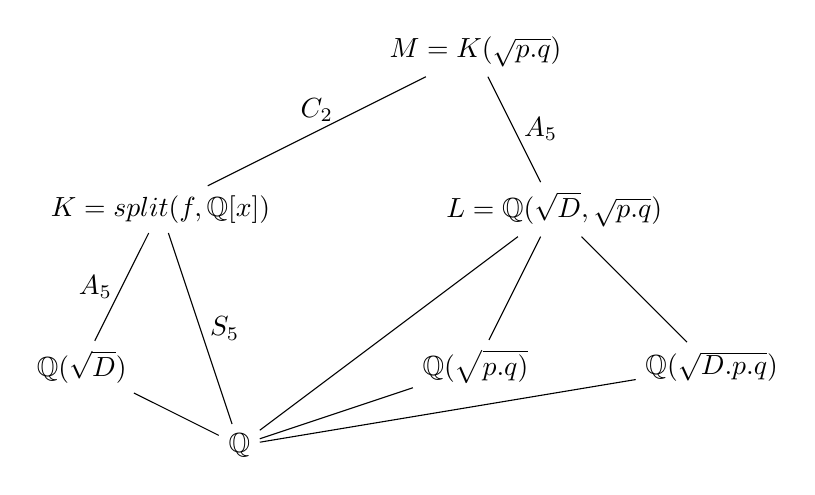
\begin{tikzpicture} [align=center]
  \path  (0, 0)   node(Q)  {$\mathbb{Q}$}
          +(6, 1)   node(QD12) {$\mathbb{Q}(\sqrt{D.p.q})$}
          ++(3,1)   node(Q12) {$\mathbb{Q}(\sqrt{p.q)}$}
           ++(-5,0)   node(QD) {$\mathbb{Q}(\sqrt{D})$}
           ++(1,2)   node(K) {$K=split(f,\mathbb{Q}[x])$}
           ++(5,0)   node(L) {$L=\mathbb{Q}(\sqrt{D},\sqrt{p.q})$}
            ++(-1,2)   node(M) {$M=K(\sqrt{p.q})$};
    \draw [-] (Q) to node [pos=0.5,above]{} (Q12);
    \draw [-] (Q) to node [pos=0.8,below]{} (QD);
    \draw [-] (Q) to node [pos=0.5,below]{} (QD12);
  \draw [-] (QD) to node [pos=0.5,left]{$A_5$} (K);
  \draw [-] (Q) to node [pos=0.5,right]{$S_5$} (K);
  \draw [-] (Q) to node [pos=0.5,below]{} (L);
  \draw [-] (Q12) to node [pos=0.5,below]{} (L);
  \draw [-] (QD12) to node [pos=0.5,below]{} (L);
    \draw [-] (L) to node [pos=0.5,right]{$A_5$} (M);
     \draw [-] (K) to node [pos=0.5,above]{$C_2$} (M);
\end{tikzpicture}
\end{center}  
\end{frame}

\begin{frame}{Examples of Suitable Polynomials and Primes}
  Using SageMath, the following polynomial and primes were found:
\begin{example}
$f(x)=x^5+4x^4-6x^2-x+1, p=1531,q=71,151,227,\Delta(f)=170701$
\end{example}
    \begin{example}
$ f(x)=x^5-4x^4+12x^2-8x+1,p=1987,q=31,107,211,239,\Delta(f)=186037$
\end{example}
These polynomials satisfy the criteria of the above theorem and therefore describe fields with infinite unramified extensions. Furthermore, the class number of the splitting fields of each of these polynomials is 1, meaning that they are equal to their own Hilbert class fields.  
\end{frame}

\end{document}
